\chapter{Przegląd dziedziny}
Rozdział ten zawiera opis kilku wybranych bibliotek służących do tworzenia wykresów. Opisałem tu  biblioteki przeznaczone dla Qt i~C++, podzielone na rozwiązania komercyjne oraz darmowe. Dla każdej biblioteki podałem jej zalety i~wady. Następnie przedstawiam wykaz typów wykresów dostępnych we wszystkich opisanych produktach. Kolejne dwa paragrafy to zestawienie elementów wspólnych i~unikalnych. Ostatni fragment to podsumowanie zawierające wnioski płynące z~tego przeglądu.

\section{Rozwiązania komercyjne}
Istnieje kilka komercyjnych bibliotek służących do tworzenia wykresów w~Qt. Zostały one stworzone przez najpoważniejsze studia developerskie tworzące oprogramowanie w~Qt. Bliższe przyjrzenie się tym bibliotekom pomogło mi stworzyć listę wymagań stawianych mojej bibliotece oraz częściowo zasugerowało pewne rozwiązania strukturalne.
 
\subsection{Qt Commercial Charts}
Biblioteka ta została stworzona przez aktualnego właściciela Qt, czyli firmę Digia. Oferuje ona programiście szeroki wybór wykresów. Nie wymaga zagłębiania się w~swoją wewnętrzną budowę, a~tworzenie prostych wykresów polega na połączeniu kilku wysokopoziomowych obiektów takich jak seria czy widget widoku.\newline

Cała biblioteka opiera się na frameworku Graphics View, który wprowadza podział na scenę oraz widok, gdzie scena jest kontenerem na elementy prezentowane za pomocą widoku.
Biblioteka udostępnia dwa uniwersalne widoki. Zależnie od zastosowania można użyć obiektu klasy dziedziczącej z~QGraphicsView bądź z~QGraphicsWidget. Implementacje konkretnych wykresów zarządzają elementami dodawanymi do sceny.\newline

Biblioteka ta, jako jedyna z tutaj opisanych, udostępnia wszystkie swoje wykresy w~języku QML, zarówno dla QtQuick~1~i~2.
Jak sam producent zaznacza, silne uzależnienie biblioteki od GraphicsView sprawia, że osiąga ona lepsze wyniki wydajnościowe dla QtQuick~1.\newline

\textbf{Zalety:}
\begin{itemize}
\item{szeroki wybór wykresów,}
\item{operowanie na komponentach wysokiego poziomu,}
\item{interaktywność wszystkich elementów wykresu,}
\item{system motywów umożliwiający tworzenie wykresów o~spójnej kolorystyce,}
\item{obiekty mapujące dane ze standardowych modeli Qt do serii danych,}
\item{wtyczka do Designera,}
\item{silne wsparcie dla QML.}\newline
\end{itemize}

\textbf{Wady:}
\begin{itemize}
\item{spadek uniwersalności poprzez uzależnienie prezentacji wykresów od konkretnych widoków,}
\item{wykorzystanie GraphicsView zamiast SceneGraph, powodujące niższą wydajność w QtQuick~2.}
\end{itemize}


\subsection{KD Charts}
Jest to biblioteka stworzona przez firmę KDAB. KD Charts w~odróżnieniu od poprzedniej biblioteki nie korzysta z~GraphicsView, a~z~mechanizmów niższego poziomu. Rysowanie odbywa się tu za pomocą systemu Arthur, a~do pisania wykorzystano silnik Scribe.
Dzięki wykorzystaniu technologii niższego poziomu, programistom KDAB udało się uzyskać lepszą wydajność, szczególnie ważną przy oferowanych przez nich wykresach czasu rzeczywistego.\newline

KD Charts separuje dane od warstwy prezentacji wykorzystując modele znane z~popularnego w~Qt wzorca Model-Widok. Za prezentację danych odpowiada uniwersalna klasa dziedzicząca po QWidget.\newline

\textbf{Zalety:}
\begin{itemize}
\item{szeroki wybór wykresów,}
\item{zbiór wbudowanych interakcji oraz możliwość tworzenia własnych,}
\item{duże możliwości parametryzowania wyglądu wykresu,}
\item{wykresy 2,5D,}
\item{wysoka wydajność, umożliwiająca tworzenie wykresów czasu rzeczywistego.}\newline
\end{itemize}

\textbf{Wady:}
\begin{itemize}
\item{wysoka cena,}
\item{wymuszenie korzystania z~modeli albo niskopoziomowych kontenerów do przechowywanie danych,}
\item{biblioteka napisana w~stylu Qt4, trudnym do wykorzystania w~QtQuick~2,}
\item{brak wsparcia dla QML.}
\end{itemize}

\subsection{QtitanChart}
Jest to biblioteka stworzona przez firmę Developer Machines, udostępniająca dosyć duży zbiór wykresów. Twórcy biblioteki nie udostępniają pełnych źródeł swojej biblioteki, a~jedynie jej pliki nagłówkowe i~biblioteki dynamiczne, co znacznie utrudnia zrozumienie jej wewnętrznego działania. Ta wiedza nie jest jednak potrzebna, gdyż aby tworzyć za jej pomocą wykresy, można się posługiwać komponentami wysokiego poziomu.\newline

\textbf{Zalety:}
\begin{itemize}
\item{szeroki wybór wykresów,}
\item{możliwość wyeksportowania wykresu do pliku graficznego,}
\item{możliwość wyświetlania wykresów różnych typów w~jednym układzie współrzędnych,}
\item{system motywów, umożliwiający tworzenie wykresów o~jednolitej kolorystyce.}\newline
\end{itemize}

\textbf{Wady:}
\begin{itemize}
\item{wysoka cena,}
\item{brak wsparcia dla QML.}
\end{itemize}


\section{Rozwiązania darmowe}
Warto również przyjrzeć się bibliotekom open--source, choćby po to, aby wiedzieć jakich rozwiązań unikać w~czasie projektowania mojej biblioteki.

\subsection{Qwt}
Qt Widgets for Technical Applications to otwarta biblioteka umożliwiająca tworzenie wykresów oraz innych widgetów technicznych. Biblioteka ta była projektowana z~myślą o zastosowaniach technicznych, w~szczególności w~systemach czasu rzeczywistego, przez co głównym celem było zapewne osiągnięcie wysokiej wydajności przy dynamicznie zmieniających się danych. Cel ten osiągnięto między innymi poprzez wykorzystywanie stosunkowo niskopoziomowych mechanizmów, jak Arthur czy intensywne wykorzystanie szablonów języka C++. Niestety przez to biblioteka nie jest szczególnie przyjazna użytkownikowi. Programista często musi sięgać do niskopoziomowych narzędzia, a stworzenie mniej standardowego rozwiązania może sprawić wiele trudności.\newline

Qwt zawiera szerokie API służące do przeprowadzania różnorakich operacji na wykresach, m.in. skalowania i zaznaczania. Problematyczną kwestią jest wygląd wykresów, z~jednej strony są one adekwatne dla zastosowań technicznych, z~drugiej zaś sprawia on, że nie sposób użyć tych wykresów w~aplikacji innego typu, ze względu na ich brzydotę. Najlepszym przykładem niech będzie wykres załączony na rys. \ref{rys:wykres:sinus}, wyglądający niczym oscylogram.
\begin{figure}
\centering
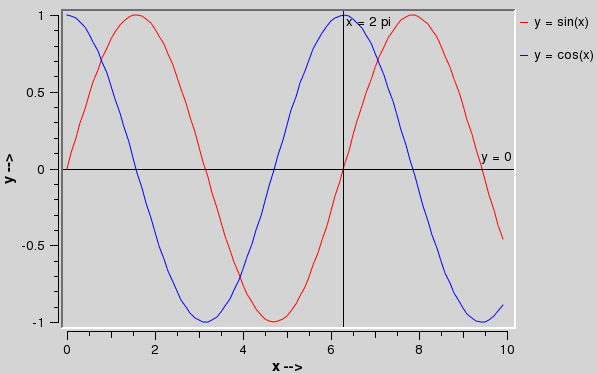
\includegraphics[scale=0.4]{img/sinus.png}
\caption{Przykładowy wykres Qwt}\label{rys:wykres:sinus}
\end{figure}

\textbf{Zalety:}
\begin{itemize}
\item{rozbudowane API,}
\item{wsparcie społeczności,}
\item{wysoka wydajność,}
\item{osie ze skalą logarytmiczną.}\newline
\end{itemize}

\textbf{Wady:}
\begin{itemize}
\item{nieprzyjazna użytkownikowi,}
\item{mało atrakcyjny wygląd wykresów,}
\item{brak wsparcia dla QML.}
\end{itemize}

\subsection{GobChartWidget}
Jest to jednoosobowy projekt rozwijany przez Williama Hallatta, dostępny na licencji open-source. Biblioteka ta ma bardzo ograniczoną funkcjonalność, pozwala na tworzenie wykresów tylko trzech typów: słupkowych, liniowych oraz kołowych, wszystkie o~bardzo prostym wyglądzie.\newline

Jest to kolejna biblioteka uzależniona od frameworku Model-Widok. Jest to jednak przypadek ekstremalny, nie polegający jedynie na trzymaniu danych w~modelu. Klasy odpowiedzialne za prezentację wykresów dziedziczą tu po abstrakcyjnym widoku z~ww. frameworku. Zapewne twórca uzyskał dzięki temu pewne ciekawe własności, jednak zmusiło go to do implementacji osobnych widoków dla każdego typu wykresu.\newline

Do rysowania wykresów wykorzystano tu GraphicsView, przy czym kontenerem na elementy nie jest scena, a~model.\newline

Jak widać GobChartWidget jest nieco dziwną hybrydą, której z~pewnością nie można nazwać skalowalną. Wcale nie dziwi fakt, że nie cieszy się ona szczególną popularnością wśród programistów Qt. Według statystyk SourceForge~\footnote{SourceForge \url{http://sourceforge.net}}, w~ciągu pół roku pobrano tę bibliotekę zaledwie kilkanaście razy.

\textbf{Zalety:}
\begin{itemize}
\item{darmowa,}
\item{najpopularniejsze wykresy,}
\item{współpraca z systemem Model-Widok}\newline
\end{itemize}

\textbf{Wady:}
\begin{itemize}
\item{ubogi zbiór wykresów,}
\item{mało przejrzysta struktura,}
\item{brak wspierającej społeczności programistów,}
\item{brak wsparcia dla QML.}
\end{itemize}



\section{Dostępne typy wykresów}
Podstawowym kryterium oceny użyteczności tego typu biblioteki jest zbiór wykresów, które udostępnia. Tablica~\ref{tab:wykresy} prezentuje dostępność typów wykresów w~opisanych bibliotekach. Podstawową informacją wynikającą z~tego zestawienia jest fakt, że najpopularniejsze są wykresy kołowy, słupkowy oraz liniowy.
\begin{table}[h]\footnotesize
\centering
\caption{Zestawienie dostępnych wykresów}
\label{tab:wykresy}
\begin{tabular}{|c|c|c|c|c|c|}
\hline
&  Qt Charts & KD Chart & Qtitan & Qwt & GobChart\\
\hline
Bąbelkowy & T & N & T & N & N\\
\hline
Gantta & N & T & N & N & N\\
\hline
Kołowy & T & T & T & N & T\\
\hline
Liniowy & T & T & T & T & T\\
\hline
Pierścieniowy & T & T & T & N & N\\
\hline
Słupkowy & T & T & T & N & T\\
\hline
Świecowy & T & T & N & N & N\\
\hline
Warstwowy & T & T & T & N & N\\
\hline
XY (punktowy) & T & N & T & T & N\\
\hline
\end{tabular}
\end{table}


\section{Elementy wspólne}
Analizując powyższe biblioteki dochodzę do wniosku, że można wykroić z nich część wspólną, stanowiącą podstawową funkcjonalność niezbędną dla biblioteki tego typu. Te elementy to:
\begin{itemize}
\item{podstawowe wykresy, takie jak liniowy, słupkowy i kołowy,}
\item{osie, siatka i legenda,}
\item{możliwość realizacji przez programistę interakcji z~użytkownikiem,}
\item{zaznaczanie i przybliżanie fragmentów wykresu,}
\item{serie danych -- każda z bibliotek wykorzystuje ujednolicony interfejs do danych. Czesem seria jest jedynie opakowaniem na kontener z~próbkami, innym razem zawiera większość logiki związanej z~konstrukcją wykresu,}
\item{efekty 2,5-3D, komercyjne biblioteki umożliwiają tworzenie pseudo-przestrzennych wykresów.}
\end{itemize}

\section{Elementy unikalne}
Prawie wszystkie biblioteki zawierają wartościowe elementy niepowtarzalne lub rzadko spotykane:
\begin{itemize}
\item{animacja towarzysząca tworzeniu wykresów oraz ich przebudowywaniu,}
\item{motywy pozwalające na tworzenie wykresów w~różnych, jednolitych stylach,}
\item{możliwość realizacji pełnej interakcji ze wszystkimi elementami wykresu,}
\item{możliwość konfiguracji elementu prezentującego kolor w~legendzie (np. koło dla wykresu bąbelkowego, odcinek dla liniowego),}
\item{generowanie plików graficznych zawierających wykresy,}
\item{możliwość wyświetlania kilku wykresów różnego typu w~jednym układzie współrzędnych,}
\item{możliwość korzystania z~nieliniowych skal osi przy wykresach osadzonych w~układzie współrzędnych,}
\item{wyeksponowanie klas C++ w QML.}
\end{itemize}

\section{Podsumowanie}
Na rynku istnieją już wartościowe biblioteki pozwalające na tworzenie wykresów biurowych, są to jednak rozwiązania komercyjne. Projekty open-source są albo niskiej jakości albo nadają się do innych (technicznych) zastosowań. Istnieje więc potrzeba stworzenia wysokiej jakości darmowego produktu, który zyskałby taką popularność jak Qwt. Potrzeba ta jest jeszcze większa dla Qt~Quick, gdzie nie ma żadnych darmowych bibliotek pozwalających na tworzenie wykresów.

Warto również zauważyć, że twórcy żadnej z~opisanych bibliotek nie zdecydowali się na pełne odizolowanie silnika biblioteki od widoków. Dzięki takiemu podejściu osiągnąłem możliwość wyświetlania wykresów w dowolnym miejscu -- wewnątrz widgetu, w~aplikacji napisanej w~QML czy w~dokumencie tekstowym. Jest to pierwsze takie rozwiązanie na rynku.


